\section{Methods} 

\subsection{Test Protocol} 

There are several sources and databases on human gait data, for example, the Winter database \cite{winter1984kinematic}. This paper adds additional data of people climbing different stair heights to this existing library of human motion data. High-resolution data of human motion is required to learn a stair climbing trajectory. It enables researchers to build and develop complex mechanisms such as orthosis and exoskeletons \cite{moore2015elaborate}.  The trial conducted collected demonstrations of how people climb stairs. The Vicon system recorded the marker positions. Eleven able-bodied subjects participated in the study (5F, 6M). The Institutional Review Board of Worcester Polytechnic Institute approved the study, and each subject gave written consent. The data was anonymous, so the subjects could not be identified. \autoref{tab:subjects} holds the metadata of the subjects. All the data was saved in an ASCII format file. The custom open-source software package parses the data. The installation instructions can be found in \autoref{sec:conclusion}.

\begin{table}[h!]
\centering
 \begin{tabular}{|c c c c c|} 
 \hline 
 \multicolumn{5}{|c|}{Subjects} \\
 \hline
 ID & Mass ($Kg$) &  Height($m$)  & Age($yr$)  & Gender \\ [0.5ex] 
 \hline\hline
 0 & 59 & 1.6 & 20 & F \\
 \hline
 1 & 62 & 1.7 & 20 & F \\ 
 \hline
 2 & 86 & 1.9 & 44 & F \\
 \hline
 3 & 64 & 1.8 & 20 & M \\ 
 \hline
 4 & 50 & 1.5 & 20 & F \\
 \hline
 5 & 96 & 1.6 &  19 & F\\
 \hline
 6 & 77 & 1.8 & 22 & M \\
 \hline
 7 & 78 & 1.8 & 22 & M \\
 \hline
 8 & 95 & 1.7 & 33 & M \\
 \hline
 9 & 85 & 1.8 & 21 & M \\
 \hline
 10 & 68.5 & 1.7 & 22 & M \\[1ex] 
 \hline
\end{tabular}
\caption{The subjects' meta data recorded at the time of trial.}
\label{tab:subjects}
\end{table}

The mocap trial used a Vicon Vantage V5 system with ten cameras running at $100Hz$. The markers were placed on the subject according to the advanced Plug-in gait template \footnote{https://docs.vicon.com/display/Nexus28/Plug-in+Gait+lower+body+forces+and+moments}. Additional rigid body plates were placed on the thighs, shanks, and back of the participants for redundancy and to mitigate marker occlusion. The marker placement was calibrated to each subject prior to the study. This allowed for the measurement of the limb segments. Markers were placed on each step of the staircase and on the floor to record their positions. \autoref{fig:markers} and \autoref{fig:mocap} illustrate the marker layout and the setup used during the trial. The subjects approached the staircase, paused, and climbed the stairs with their leading leg. Each subject was allowed to climb at their own pace. Each subject repeated the action three times for each of the four different stairs of different heights. The stair heights are given in \autoref{tab:stairs}. This ensured that a good sample trial with no marker occlusion was collected.   
\begin{table}[h!]
\centering
 \begin{tabular}{||c c ||} 
 \hline
 Config & stair height (inch) \\ [0.5ex] 
 \hline\hline
 0 & 5.25  \\ 
 \hline
 1 & 6.0  \\
 \hline
 2 & 6.75  \\
 \hline
 3 & 7.5 \\
 \hline
\end{tabular}
\caption{Stair Height Configuration}
\label{tab:stairs}
\end{table}


\begin{figure}
\centering 
\begin{subfigure}{0.5\linewidth} 
  \centering 
  \includegraphics[scale=0.04,frame]{images/marker_side_cap.png} 
  \caption{Side view of the markers} 
  \label{fig:markers_side} 
\end{subfigure} 

\begin{subfigure}{0.5\linewidth} 
  \centering 
  \includegraphics[scale=0.04,frame ]{images/front_markers_cap.png} 
  \caption{Front view of the markers} 
  \label{fig:markers_front} 
\end{subfigure} 
\caption{The markers were placed according to the plugin marker template. Additional rigid body plates were placed on the subjects' thighs, shanks, feet, and back.} 
\label{fig:markers} 
\vspace*{-3mm}
\end{figure} 


\begin{figure}
    \centering 
    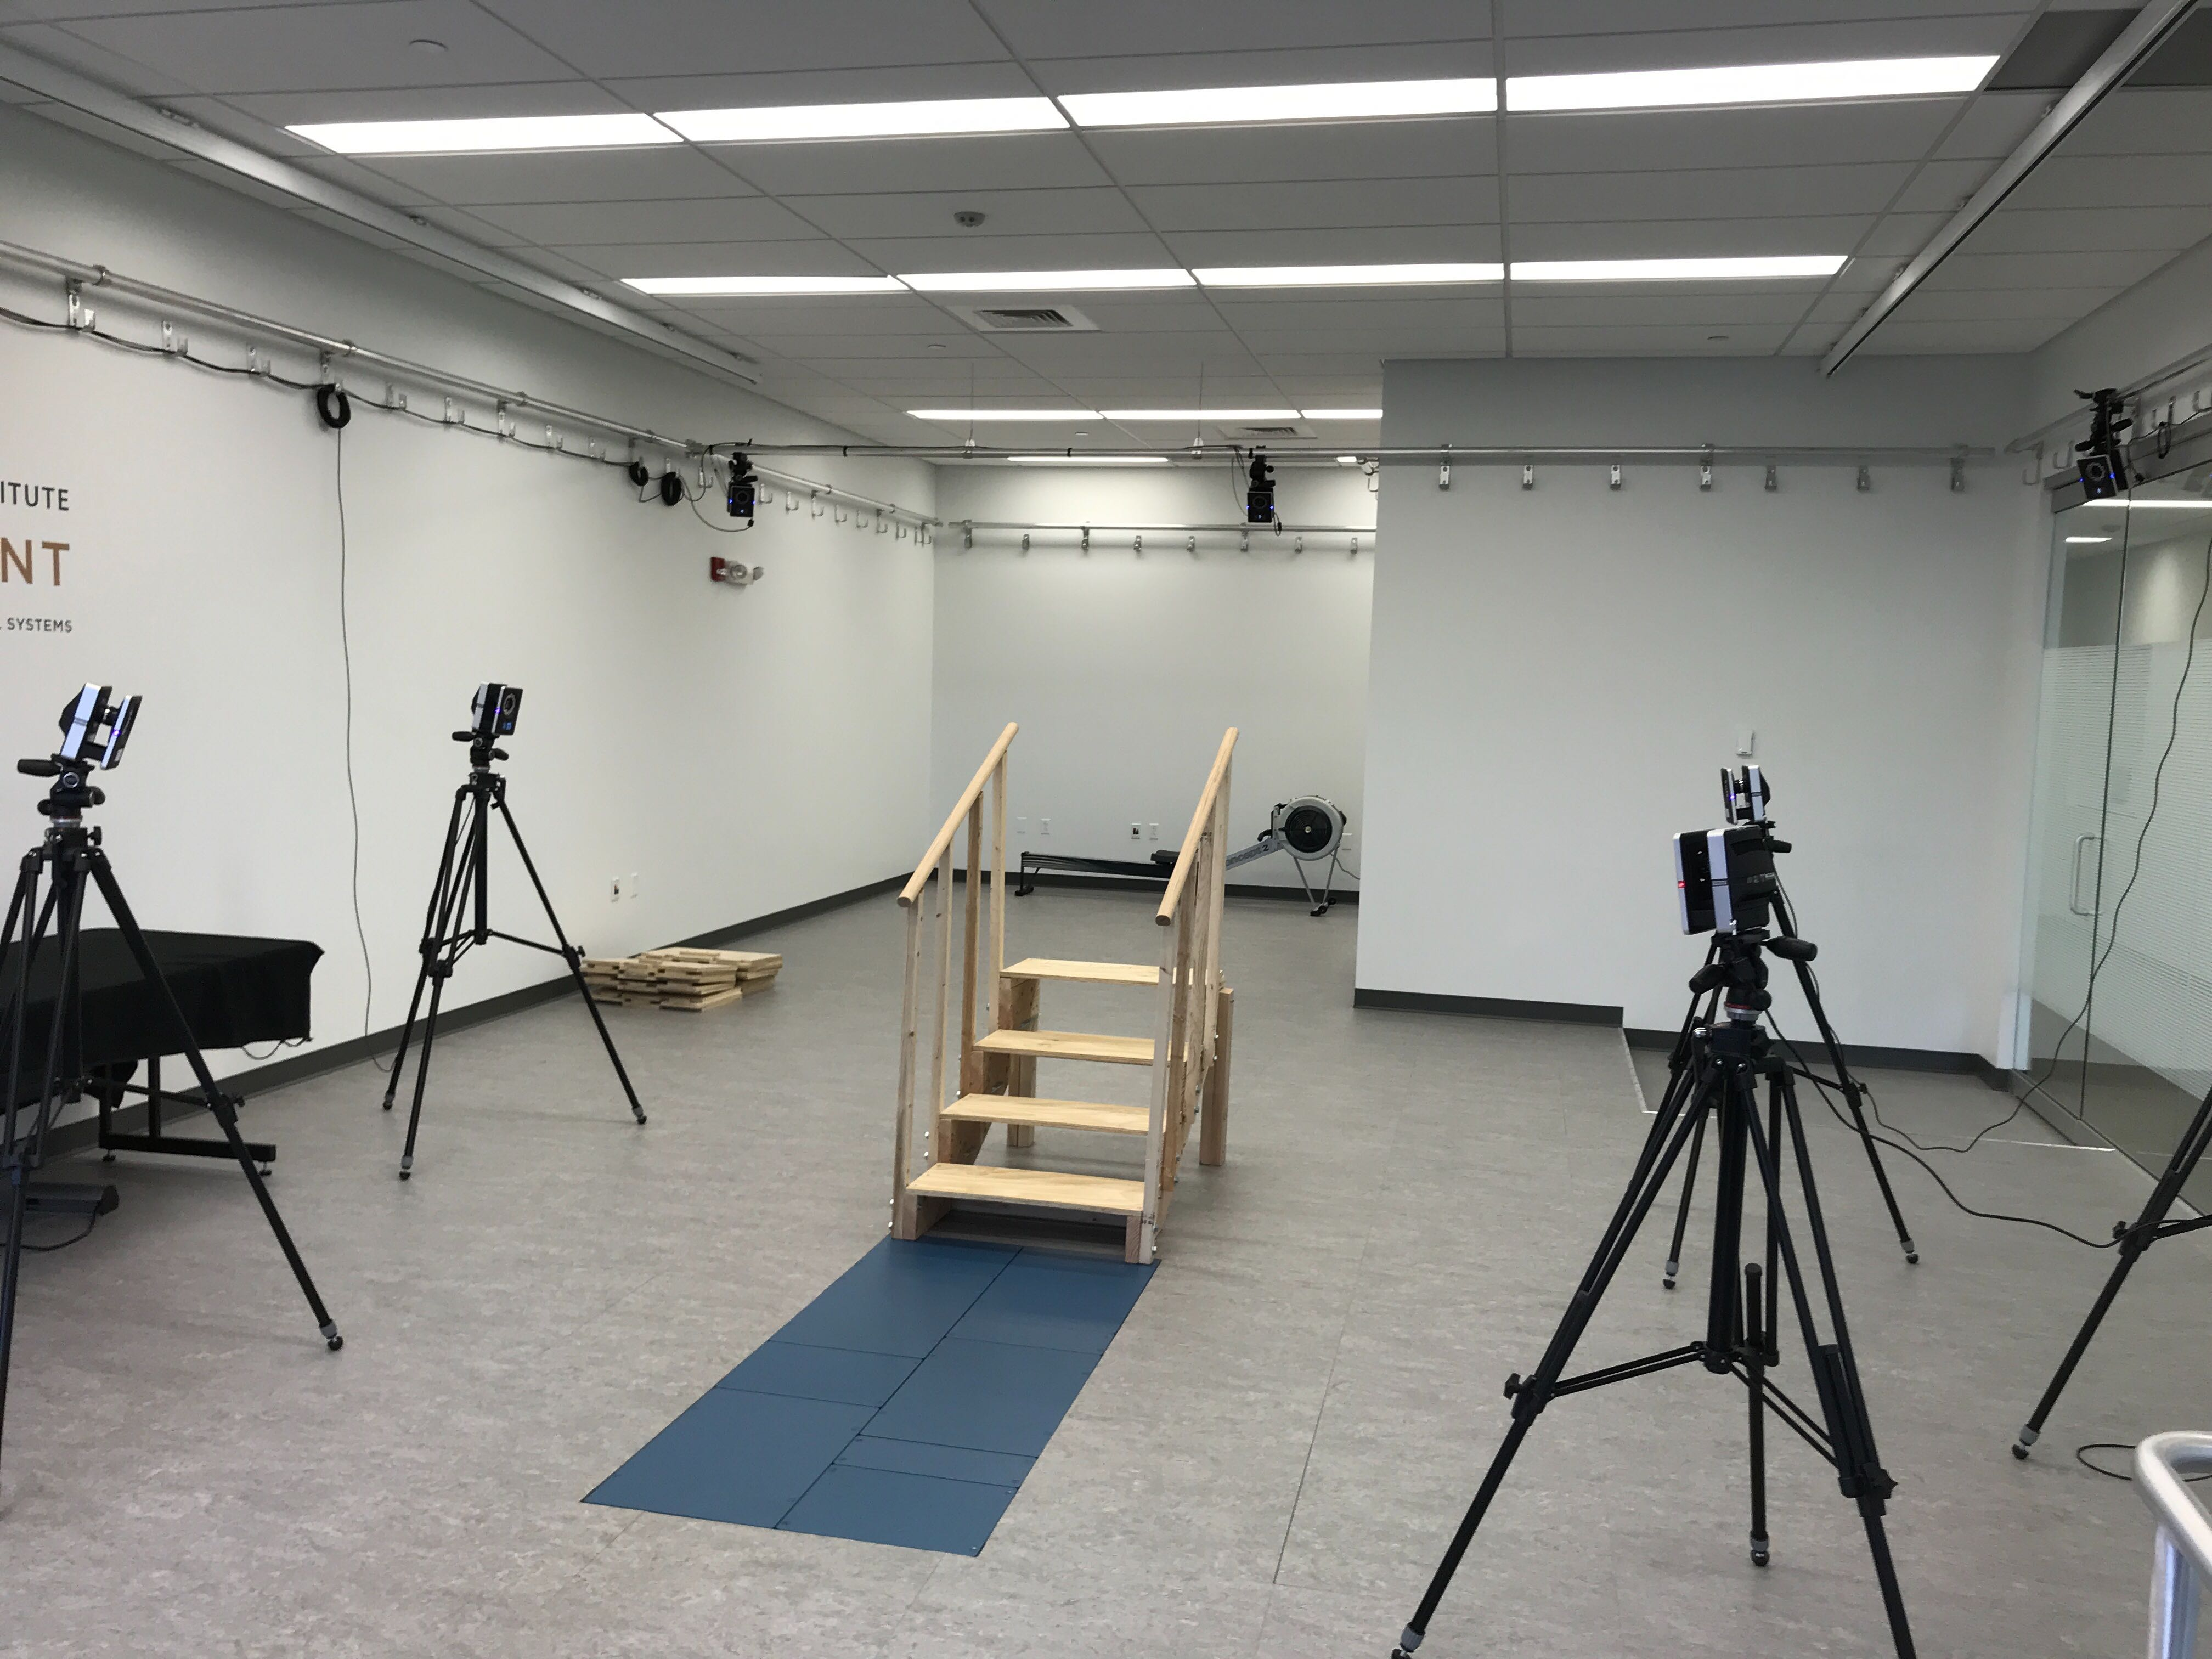
\includegraphics[scale=0.04,frame]{images/stairs.png}
    \caption{Motion capture area with custom staircases. The stairs had sliding planes to adjust the heights. Four of the mocap cameras were placed around the stairs to mitigate. marker occlusions}
    \label{fig:mocap} 
\end{figure} 

\subsection{Learning the Trajectories} 
\autoref{fig:stick} shows the coordinate layout used in this paper. The $X$ axis is perpendicular to the plane and is not considered. Exoskeletons are typically controlled in the sagittal plane, so out-of-plane motion is not required. \autoref{fig:stick} shows a diagram of the subject in motion. In this diagram, the toe's position is being controlled from the ground to the first step of the staircase. The limb lengths of the subject used for training were measured using a calibration phase. However, the limb length segments can be estimated using the height of the subject \cite{anthropomorphic}. It is assumed that the relative location of the stairs is known with respect to the person. The motion has to be transferred to joint space using inverse kinematics of the leg. To avoid a collision of the toe with the lip of the stairs, a constraint that the foot has to be parallel to the ground is imposed. In addition, some rehabilitation exoskeletons do not have actuated ankle joints and therefore cannot be controlled.  \autoref{eq:IK} is the inverse kinematics of the leg with a constrained ankle where hip: $q_1$, knee: $q_2$, ankle: $q_3$, thigh: $l_1$, shank: $l_2$, ankle height: $l_3$, foot length: $l_4$, and $z_{toe}$ and $y_{toe}$ is the coordinate of the toe. As opposed to forward kinematics, inverse kinematics allows for the encoding of the stair height. 

\begin{equation} 
    \begin{aligned} 
        y' &= y_{toe} - l_4 \\ 
        z' &= z_{toe} + l_3 \\  
        \gamma &= y'^2 - z'^2 - l_1^2  - l_2^2 \\ 
        q_2 &= atan2 \Bigg( -\sqrt{1 - \frac{\gamma }{2 l_1^2 l_2^2}}, \frac{\gamma}{2 l_1^2 l_2^2}\Bigg)\\ 
        q_1 &= (atan2(z, y) - atan2( l_2 s_{q_2}, l_1 + l_2 c_{q_2})) + 0.5\pi \\ 
        q_3 &= (2\pi - q_1 - q_2) 
    \end{aligned} 
    \label{eq:IK} 
\end{equation} 

 
\begin{figure} 
    \centering 
    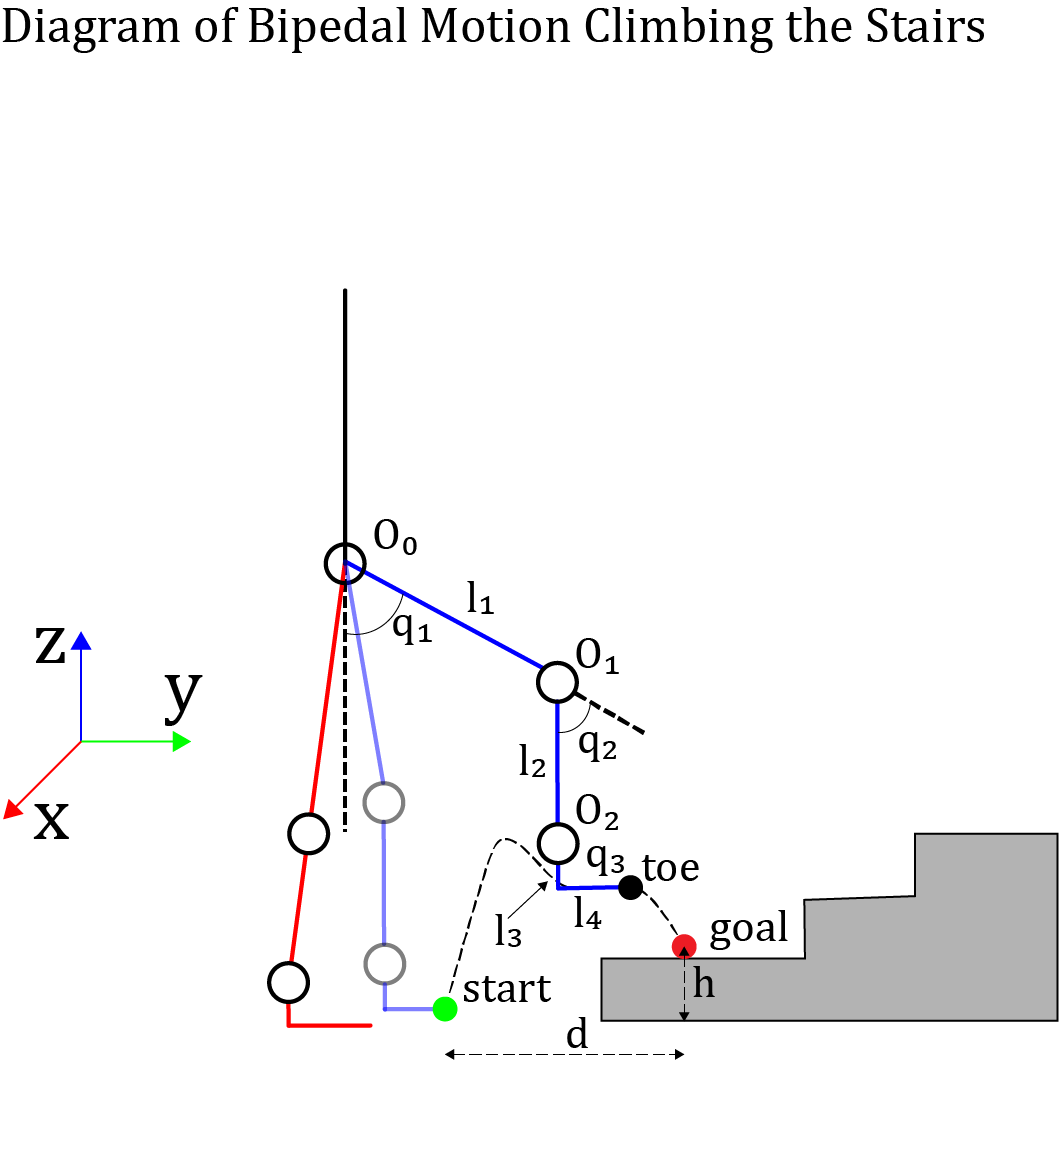
\includegraphics[scale=0.75]{images/stick.png} 
    \caption{Stair climbing motion of a 3 DoF leg. The start and goal are the parameters of the model shown as the distance $d$ and height $h$ from the toe to the stair. Each of the joint angles are calculated using inverse kinematics.} 
    \label{fig:stick} 
    \vspace*{-4mm}
\end{figure} 



Dynamic Time Warping temporally aligns two demonstrations. DTW attempts to minimize the distance between two trajectories by drawing lines between the two curves \cite{muller2007dynamic} \cite{JSSv031i07}. \autoref{eq:DTW} shows the equation for DTW; it maps demo 2 onto demo 1. Here, $\delta (P, T)$ is defined as the Manhattan distance function. $P$ and $T$ are demo 2 and demo 1, respectively. This method maps $P$ onto $T$. The Euclidean distance and Manhattan distance were both examined as criteria. Here, $w_k$ is the cost at index $(i,j)$, and $k$ is the time frame. DTW does not produce smooth trajectories; the trajectories have to be smoothed so that the derivative of the trajectory can be found. A high order polynomial fit to the temporally scaled demonstrations removes the disturbance from the demonstrations.



\begin{equation} 
    \begin{aligned} 
         \delta (P,T) &= | p_i - t_j| & \text{Distance function} \\ 
        DTW(P,T) &= min \Bigg[ \sum_{k=1}^{K} \delta (w_k) \Bigg] & \text{Minimum path} 
    \end{aligned} 
    \label{eq:DTW} 
\end{equation} 


DMPs work by encoding the force profile during the trajectory. The first and second derivative of the marker trajectory is calculated to transfer the marker trajectory from position space to a forced space using a PD controller seen in \autoref{eq:force}. The gain matrices are $K_p$ and $K_d$, $g$ is the goal of the system, and $x$ is the system state. This conversion is done because the DMP controller needs a force input to drive the system.

\begin{equation}
    F = \ddot{x} - K_p (g - x) - K_d\dot{x}
    \label{eq:force}
\end{equation}



The Expectation-Maximization (EM) algorithm iteratively updates the probabilities of the points. The EM algorithm is used to find the optimal mean and covariance of each of the Gaussian. The goal of the EM algorithm is to find similar points in the demonstrations and group them together into clusters. \autoref{eq:Estep} and \autoref{eq:Mstep} show the two steps in the EM algorithm. In these equations, $X$ is the point vector, $h$ is the posture probability, $\pi$ is the weighting coefficient for each point, $\mu$ is mean, and $ \Sigma $ is the co-variance.  K-means is used to find the initial guess of the $\mu$ and $\Sigma$ parameters for the EM algorithm with the value of $\pi$ initialized randomly. The GMM/GMR code used in this paper were based on Calinon open-source libraries \cite{Calinon19MM} \cite{CalinonLee19} \cite{Calinon16JIST}. 

E(xpectation)-step: 
\begin{equation} 
     h_{t,i} = \frac{\pi_i \prod_{j=1}^{P} \mathcal{N}(X_t^j | \mu_i^j , \Sigma_i^j )}{ \sum_k^K \pi_k \prod_{j=1}^{P} \mathcal{N}(X_t^j | \mu_k^j , \Sigma_k^j ) } 
     \label{eq:Estep} 
\end{equation}{} 

M(aximization)-step: 
\begin{equation} 
\begin{aligned} 
    \pi_i &\leftarrow \frac{\sum_t^N h_{t,i}}{N} \\ 
    \mu_i^j &\leftarrow \frac{\sum_t^N h_{t,i} X_t^j}{\sum_t^N h_{t,i}} \\ 
    \Sigma_i^j &\leftarrow \frac{\sum_t^N h_{t,i} ( X_t^j - \mu_i^j)  ( X_t^j - \mu_i^j)^T   }{\sum_t^N h_{t,i}}  
\end{aligned} 
\label{eq:Mstep} 
\end{equation} 


The number of bins $ K $ can be found using the Bayesian Information Criterion (BIC). If too few bins are used, the model will be poorly fit; if too many are used, it will over-fit to the demonstrations. BIC is a method to overcome this limitation and find the optimal number of bins. \autoref{eq:BIC} calculates the BIC score; it is a trade-off between optimizing the likelihood and minimizing the number of states to encode.  $\mathcal{L}$ is the log-likelihood, $ N $ is the number of mixture models, $ K $ is the number of components, and $ D $ is the dimension of the data points. \cite{calinon2007learning, billard2006discriminative}. 


\begin{equation} 
    S_{BIC} = -\mathcal{L} + \frac{log(N)(K(D+1)(D+2)-2)}{4}  
    \label{eq:BIC} 
\end{equation} 





GMR models the regression function from the joint probabilities in the form of GMM. The GMM algorithm is a probabilistic form of the K-means algorithm. In this formulation, GMM was used to find the mean and covariance of the basis functions over the data set. GMR was used to regress over the basis function, creating the forcing function needed for the DMP. \autoref{eq:GMR_Prop} calculates the likelihood and \autoref{eq:GMR_mu} calculates the covariance and mean. $\xi_$ is a multidimensional array, $\mu_i^o$ and $\Sigma_t^o$ are vectors of the output mean and covariance, and $\mu_i^I$ and $\Sigma_t^I$ are vectors of the input mean and covariance.   \autoref{fig:GMM} shows the position of the Gaussian and force profile. There are several Gaussian on the upper graph; some are easily visible. The others have small eigenvalues, creating an eclipse with small areas. The blue lines are the training force profiles, with the red line being the learned force profile.   

\begin{equation} 
     P(\xi_t^O | \xi_t^I ) \sim \sum_i^K h_i(\xi_t^I) \mathcal{N}( \hat{\mu_i^o}, \hat{\Sigma_t^o}) 
     \label{eq:GMR_Prop} 
\end{equation} 

where, 

\begin{equation} 
    \begin{aligned} 
      \hat{\mu_i^o} &= \mu_i^o + \Sigma_i^{OI}\Sigma_i^{I-1}(\xi_t^I - \mu_i^I)\\ 
      \hat{\Sigma_i^O} &= \Sigma_i^O - \Sigma_i^{OI}\Sigma_i^{I-1}(\xi_t^I - \mu_i^I) \\ 
       h_{i} &= \frac{\pi_i \mathcal{N}(\xi_t^I | \mu_i^j , \Sigma_i^j )}{ \sum_k^K \pi_k \mathcal{N}(\xi_t^I | \mu_k^j , \Sigma_k^j ) }   
    \end{aligned} 
    \label{eq:GMR_mu} 
\end{equation} 

DMPs allow for the manipulation of the encoded trajectories. \autoref{eq:DMP} shows the basic formulation of the DMPs. The force function $f$ is calculated from GMR and drives the function, $\beta_y$ and $\alpha_y$ are the system gains, $y$ is the system state, and $g$ is the goal. \autoref{eq:canonical} shows the canonical system. $\tau$ is a time constant and $\alpha_x$ is a constant term. It models the generic behavior of the model. The $\tau$ term is used for scaling the trajectories in time.  


\begin{equation}
    \tau \ddot{y} = \alpha_x (\beta_y(g-x)-\dot{y}) + f  
    \label{eq:DMP} 
\end{equation}


\begin{equation}
    \tau \dot{x} = -\alpha_x x  
    \label{eq:canonical} 
\end{equation}



A reproduction model's accuracy can be measured by calculating the imitation cost. This is essentially a root mean squared algorithm that measures how well the model follows the demonstrations \cite{metric}. \autoref{eq:metric} shows the equation used to calculate the goodness of fit. In this equation, $d$ is the demo, $m$ is each of the demos, $t$ is the time, and $x$ is the trained model. All of the demonstrations were first aligned using DTW.

   \begin{equation}
        C = \frac{1}{MT} \sum_m^M{\sum_t^T{ || d^m_t - x_t||}}
        \label{eq:metric}
    \end{equation}


